\documentclass[fleqn,10pt]{latex/stylish_article} % Document font size and equations flushed left

\setcounter{tocdepth}{3}

% Pandoc environments
\usepackage{framed}
\usepackage{fancyvrb}
\providecommand{\tightlist}{%
  \setlength{\itemsep}{0pt}\setlength{\parskip}{0pt}}
\newcommand{\VerbBar}{|}
\newcommand{\VERB}{\Verb[commandchars=\\\{\}]}
\DefineVerbatimEnvironment{Highlighting}{Verbatim}{commandchars=\\\{\}, fontsize=\scriptsize} % R Code

% Colored code
\usepackage{color}
\definecolor{shadecolor}{RGB}{248,248,248}
\newenvironment{Shaded}{\begin{snugshade}}{\end{snugshade}}
\newcommand{\KeywordTok}[1]{\textcolor[rgb]{0.13,0.29,0.53}{\textbf{{#1}}}}
\newcommand{\DataTypeTok}[1]{\textcolor[rgb]{0.13,0.29,0.53}{{#1}}}
\newcommand{\DecValTok}[1]{\textcolor[rgb]{0.00,0.00,0.81}{{#1}}}
\newcommand{\BaseNTok}[1]{\textcolor[rgb]{0.00,0.00,0.81}{{#1}}}
\newcommand{\FloatTok}[1]{\textcolor[rgb]{0.00,0.00,0.81}{{#1}}}
\newcommand{\ConstantTok}[1]{\textcolor[rgb]{0.00,0.00,0.00}{{#1}}}
\newcommand{\CharTok}[1]{\textcolor[rgb]{0.31,0.60,0.02}{{#1}}}
\newcommand{\SpecialCharTok}[1]{\textcolor[rgb]{0.00,0.00,0.00}{{#1}}}
\newcommand{\StringTok}[1]{\textcolor[rgb]{0.31,0.60,0.02}{{#1}}}
\newcommand{\VerbatimStringTok}[1]{\textcolor[rgb]{0.31,0.60,0.02}{{#1}}}
\newcommand{\SpecialStringTok}[1]{\textcolor[rgb]{0.31,0.60,0.02}{{#1}}}
\newcommand{\ImportTok}[1]{{#1}}
\newcommand{\CommentTok}[1]{\textcolor[rgb]{0.56,0.35,0.01}{\textit{{#1}}}}
\newcommand{\DocumentationTok}[1]{\textcolor[rgb]{0.56,0.35,0.01}{\textbf{\textit{{#1}}}}}
\newcommand{\AnnotationTok}[1]{\textcolor[rgb]{0.56,0.35,0.01}{\textbf{\textit{{#1}}}}}
\newcommand{\CommentVarTok}[1]{\textcolor[rgb]{0.56,0.35,0.01}{\textbf{\textit{{#1}}}}}
\newcommand{\OtherTok}[1]{\textcolor[rgb]{0.56,0.35,0.01}{{#1}}}
\newcommand{\FunctionTok}[1]{\textcolor[rgb]{0.00,0.00,0.00}{{#1}}}
\newcommand{\VariableTok}[1]{\textcolor[rgb]{0.00,0.00,0.00}{{#1}}}
\newcommand{\ControlFlowTok}[1]{\textcolor[rgb]{0.13,0.29,0.53}{\textbf{{#1}}}}
\newcommand{\OperatorTok}[1]{\textcolor[rgb]{0.81,0.36,0.00}{\textbf{{#1}}}}
\newcommand{\BuiltInTok}[1]{{#1}}
\newcommand{\ExtensionTok}[1]{{#1}}
\newcommand{\PreprocessorTok}[1]{\textcolor[rgb]{0.56,0.35,0.01}{\textit{{#1}}}}
\newcommand{\AttributeTok}[1]{\textcolor[rgb]{0.77,0.63,0.00}{{#1}}}
\newcommand{\RegionMarkerTok}[1]{{#1}}
\newcommand{\InformationTok}[1]{\textcolor[rgb]{0.56,0.35,0.01}{\textbf{\textit{{#1}}}}}
\newcommand{\WarningTok}[1]{\textcolor[rgb]{0.56,0.35,0.01}{\textbf{\textit{{#1}}}}}
\newcommand{\AlertTok}[1]{\textcolor[rgb]{0.94,0.16,0.16}{{#1}}}
\newcommand{\ErrorTok}[1]{\textcolor[rgb]{0.64,0.00,0.00}{\textbf{{#1}}}}
\newcommand{\NormalTok}[1]{{#1}}

% cslreferences environment required by pandoc > 2.7

% Polyglossia
\usepackage{polyglossia}
\setmainlanguage{en-US}
\setotherlanguage{fr-FR}
\setotherlanguage{it}

% Figures
\usepackage{graphicx,grffile}
\makeatletter
\def\maxwidth{\ifdim\Gin@nat@width>\linewidth\linewidth\else\Gin@nat@width\fi}
\def\maxheight{\ifdim\Gin@nat@height>\textheight0.8\textheight\else\Gin@nat@height\fi}
\makeatother
% Scale images if necessary, so that they will not overflow the page
% margins by default, and it is still possible to overwrite the defaults
% using explicit options in \includegraphics[width, height, ...]{}
\setkeys{Gin}{width=\maxwidth,height=\maxheight,keepaspectratio}

% Additional packages
\RequirePackage{natbib}             % Advanced Bibliography (citep...).
\RequirePackage{amsmath,amsfonts,amssymb}
\RequirePackage{breqn}              % Line breaks in equations
\RequirePackage{url}                % Line breaks in url's
\RequirePackage{enumitem}           % Line spacing in lists
  \setlist[itemize]{noitemsep,nolistsep}
  \setlist[enumerate]{noitemsep,nolistsep}

% Tables
\usepackage{longtable,booktabs}
\usepackage{caption}
% These lines are needed to make table captions work with longtable:
\makeatletter
\def\fnum@table{\tablename~\thetable}
\makeatother
% longtable 2 columns
% https://tex.stackexchange.com/questions/161431/how-to-solve-longtable-is-not-in-1-column-mode-error
\makeatletter
\let\oldlt\longtable
\let\endoldlt\endlongtable
\def\longtable{\@ifnextchar[\longtable@i \longtable@ii}
\def\longtable@i[#1]{\begin{figure}[t]
\onecolumn
\begin{minipage}{0.5\textwidth}\scriptsize
\oldlt[#1]
}
\def\longtable@ii{\begin{figure}[t]
\onecolumn
\begin{minipage}{0.5\textwidth}\scriptsize
\oldlt
}
\def\endlongtable{\endoldlt
\end{minipage}
\twocolumn
\end{figure}}
\makeatother

% Full-width tables
\usepackage{tabu}
\renewenvironment{table}{\begin{table*}}{\end{table*}\ignorespacesafterend}
  
% User-adder preamble
\hyphenation{bio-di-ver-si-ty sap-lings}

% hyperref comes last
\RequirePackage{hyperref}           % Hypertext links, PDF bookmarks
  \hypersetup{urlcolor=blue,linkcolor=black,citecolor=black,colorlinks=true}

%----------------------------------------------------------------------------------------
%	ARTICLE INFORMATION
%----------------------------------------------------------------------------------------

\JournalInfo{Publication reference} % Journal information
\Archive{DOI: xxx/xx} % Additional notes (e.g. copyright, DOI, review/research article)

\PaperTitle{Title of the Article} % Article title

\Authors{
First Author's name\textsuperscript{1*}\\ Second Author's name\textsuperscript{2}
} % Authors
\affiliation{
\textsuperscript{1}Department / University\\ \hspace{1em} Street address, Zip code, Country.\\\textsuperscript{2}Department / University\\ \hspace{1em} Street address, Zip code, Country.
}
\affiliation{*\textbf{Corresponding author}: \href{mailto:name@company.com}{\nolinkurl{name@company.com}}, \url{https://www.company.com}} % Corresponding author

\Keywords{keyword1, keyword2, etc} % Keywords
\newcommand{\keywordname}{Keywords} % Defines the keywords heading name

%----------------------------------------------------------------------------------------
%	ABSTRACT
%----------------------------------------------------------------------------------------

\Abstract{
Summary of the article.
}

%----------------------------------------------------------------------------------------

\begin{document}

\selectlanguage{en-US}

\flushbottom % Makes all text pages the same height

\maketitle % Print the title and abstract box

\tableofcontents % Print the contents section

\thispagestyle{empty} % Removes page numbering from the first page

%----------------------------------------------------------------------------------------
%	ARTICLE CONTENTS
%----------------------------------------------------------------------------------------

\hypertarget{introduction}{%
\section{Introduction}\label{introduction}}

This template allows writing articles in Markdown\footnote{\url{https://ericmarcon.github.io/travailleR/chap-rediger.html}} format.
It directly produces well-formatted articles for self-archiving (deposit on HAL for example) or in other formats, for example HTML.

\hypertarget{markdown}{%
\section{R Markdown}\label{markdown}}

Markdown is a very simple language for producing various types of documents: HTML, PDF, and Word among others.
Its documentation is available at the RStudio website\footnote{\url{http://rmarkdown.rstudio.com/articles.html}}.

Markdown is extended by Bookdown\footnote{\url{https://bookdown.org/yihui/bookdown/}}, which allows for book writing and more efficient syntax for articles.
This document is made with Markdown in RStudio: knitr processes the Markdown code, passes it to Pandoc for transformation into LaTeX, finally LateX compiles it into PDF.

\hypertarget{motivation}{%
\subsection{Motivation}\label{motivation}}

Markdown is very easy to learn.

Markdown allows you to integrate your R code for a \emph{reproducible} result.

Markdown allows to produce, without rewriting the text, a document in different formats: HTML, LaTeX or Word for example.

\hypertarget{how-to-do-it}{%
\subsection{How to do it}\label{how-to-do-it}}

In RStudio, create a new document of type Document R Markdown.
The wizard allows you to choose between different formats.

Click on \emph{From template}: from templates installed by packages.
The memoiR package templates are displayed: choose \emph{Stylish Article}.

It is better to create an RStudio project to benefit from all the possibilities: \emph{File} / \emph{New Project} then use the wizard to create a project from an existing folder.

Write the document in RStudio.

Clicking the \textbf{Knit} button in RStudio generates the document in the requested format.

\hypertarget{code}{%
\section{Code}\label{code}}

The main features of Markdown are summarized here.

\hypertarget{r-code}{%
\subsection{R code}\label{r-code}}

R code is included in code chunks:

\scriptsize

\begin{Shaded}
\begin{Highlighting}[]
\KeywordTok{head}\NormalTok{(cars)}
\end{Highlighting}
\end{Shaded}

\begin{verbatim}
##   speed dist
## 1     4    2
## 2     4   10
## 3     7    4
## 4     7   22
## 5     8   16
## 6     9   10
\end{verbatim}

\normalsize

\hypertarget{tables}{%
\subsection{Tables}\label{tables}}

The horizontal \texttt{-} and vertical separators \texttt{\textbar{}} allow you to draw a table according to Markdown syntax, but this is not the best method.

Tables can also be produced by R code.
The content of the table is in a dataframe.
The \texttt{kable()} function in the \emph{knitr} package prepares the table for display and passes the result to the \texttt{kable\_styling} function in the \emph{kableExtra} package for final formatting.

\scriptsize

\begin{longtable}[t]{rrrrl}
\caption{\label{tab:kable}Table created by R}\\
\toprule
Sepal length & Width & Petal length & Width & Species\\
\midrule
5.1 & 3.5 & 1.4 & 0.2 & setosa\\
4.9 & 3.0 & 1.4 & 0.2 & setosa\\
4.7 & 3.2 & 1.3 & 0.2 & setosa\\
4.6 & 3.1 & 1.5 & 0.2 & setosa\\
5.0 & 3.6 & 1.4 & 0.2 & setosa\\
\addlinespace
5.4 & 3.9 & 1.7 & 0.4 & setosa\\
\bottomrule
\end{longtable}

\normalsize

The caption is specified by the \texttt{caption} argument and referencing is possible because the table receives a label whose name is \texttt{tab:} followed by the name of the code snippet (table \ref{tab:kable}).
Always use the \texttt{booktabs\ =\ TRUE} argument so that the thickness of the separator lines is optimal in LaTeX.
The \texttt{bootstrap\_options\ =\ "striped"} option provides more readable tables in HTML.

In LaTeX, tables can have the width of the column and possibly span multiple pages, or use the width of the page, like table \ref{tab:Paracou}).



\scriptsize

\begin{table}

\caption{\label{tab:Paracou}Intervention table, summary of the disturbance intensity for the 4 plot treatments in Paracou.}
\centering
\begin{tabu} to \linewidth {>{\raggedright}X>{\raggedright}X>{\raggedright}X>{\raggedright}X>{\raggedright}X}
\toprule
Treatment & Timber & Thinning & Fuelwood & \%AGB lost\\
\midrule
Control &  &  &  & 0\\
T1 & DBH $\geq$ 50 cm, commercial species, $\approx$ 10 trees/ha &  &  & $[12\%-33\%]$\\
T2 & DBH $\geq$ 50 cm, commercial species, $\approx$ 10 trees/ha & DBH $\geq$ 40 cm, non-valuable species, $\approx$ 30 trees/ha &  & $[33\%-56\%]$\\
T3 & DBH $\geq$ 50 cm, commercial species, $\approx$ 10 trees/ha & DBH $\geq$ 50 cm, non-valuable species, $\approx$ 15 trees/ha & 40 cm $\leq$ DBH $\leq$ 50 cm, non-valuable species, $\approx$ 15 trees/ha & $[35\%-56\%]$\\
\bottomrule
\end{tabu}
\end{table}

\normalsize

This table contains mathematics: the \texttt{escape\ =\ FALSE} option is necessary.

Finally, the \texttt{full\_width\ =\ FALSE} option adjusts the width of the table to its content instead of occupying all the available width.
It must be \texttt{TRUE} for correct formatting of two-column tables in LaTeX.

\hypertarget{figures}{%
\subsection{Figures}\label{figures}}

\scriptsize

\begin{Shaded}
\begin{Highlighting}[]
\KeywordTok{plot}\NormalTok{(pressure)}
\end{Highlighting}
\end{Shaded}

\begin{figure}

{\centering 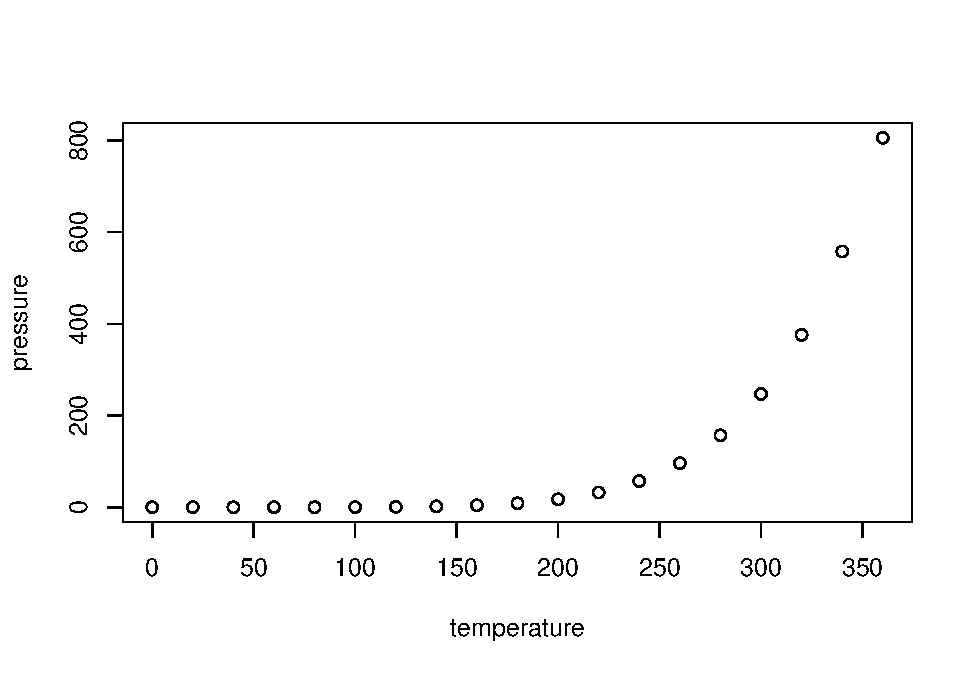
\includegraphics[width=0.8\linewidth]{/private/var/folders/24/8k48jl6d249_n_qfxwsl6xvm0000gn/T/RtmpVuR6jS/stylish_article/gallery/stylish_article/bookdown_pdf_book/stylish_article_files/figure-latex/pressure-1} 

}

\caption{Figure title}\label{fig:pressure}
\end{figure}

\normalsize

Figures can be created by the R code (figure \ref{fig:pressure}).
With Bookdown, a label is associated with each figure: its name is \texttt{fig:xxx} where \texttt{xxx} is the name of the R code snippet.
Cross-references are made with the command \texttt{\textbackslash{}@ref(fig:xxx)}.

A figure can use the full width of the page by adding the following options to the header of the code snippet that generates it: \texttt{fig.env="figure*"} and \texttt{out.extra=""}.

Existing figures are integrated into a piece of code by the \texttt{include\_graphics} function, see figure \ref{fig:logo}.

\scriptsize

\begin{figure}

{\centering 
\includegraphics[width=0.6\linewidth]{images/logo} 

}

\caption{A figure from a file}\label{fig:logo}
\end{figure}

\normalsize

Systematically place these files in the \texttt{images} folder for the automation of GitHub pages.

\hypertarget{captions}{%
\subsection{Captions}\label{captions}}

Figure and table captions can be long, include formatted text, maths, references\ldots{}
The only limit is they cannot contain more than a single paragraph.
Such captions must be stored in a separate paragraph starting with \texttt{(ref:ChunkName)}and a space.
The text of the caption follows.

In the figure chunk heading, the caption is called in the \texttt{fig.cap} field:

\{r ChunkName, fig.cap=``(ref:ChunkName)''\}

In tables, the \texttt{caption} argument of the \texttt{kable()} function is used the same way.

\hypertarget{lists}{%
\subsection{Lists}\label{lists}}

Lists are indicated by \texttt{*}, \texttt{+} and \texttt{-} (three hierarchical levels) or numbers \texttt{1.}, \texttt{i.} and \texttt{A.} (numbered lists).
Indentation of lists indicates their level: \texttt{*}, \texttt{+} and \texttt{-} may be replaced by \texttt{-} at all levels, but four spaces are needed to nest a list into another.

\begin{itemize}
\tightlist
\item
  First element of a list

  \begin{itemize}
  \tightlist
  \item
    sub-list
  \end{itemize}
\item
  Second element
\item
  Continuation of the list
\end{itemize}

Leave an empty line before and after the list, but not between its items.

\hypertarget{math}{%
\subsection{Math}\label{math}}

Equations in LaTeX format can be inserted in line, like \(A=\pi r^2\) or isolated like \[e^{i \pi} = -1\].

They can be numbered, see equation \eqref{eq:disk}, using the \texttt{equation} environment:

\begin{equation}
  A = \pi r^2.
  \label{eq:disk}
\end{equation}

\hypertarget{cross-references}{%
\subsection{Cross-references}\label{cross-references}}

Figures and tables have an automatically generated label, identical to the name of the code snippet prefixed with \texttt{fig:} and \texttt{tab:}.

For equations, the label is added manually by the code \texttt{(\textbackslash{}\#eq:xxx)} before the end of the equation.

Sections can be tagged by ending their title with \texttt{\{\#yyy\}}.

Bookmarks can also be placed freely in the text with the command \texttt{(ref:zzz)}.

In all cases, the call to the reference is made by the command \texttt{\textbackslash{}@ref(ref:zzz)}.

\hypertarget{bibliography}{%
\subsection{Bibliography}\label{bibliography}}

Bibliographic references included in the \texttt{references.bib} file can be called by \texttt{{[}@CitationKey{]}}, in parentheses \citep{Xie2016}, or without square brackets, in the text, as \citet{Xie2018} .

The bibliography is processed by Pandoc when producing Word or HTML documents.
The bibliographic style can be specified, by adding the line

\begin{verbatim}
csl:file_name.csl
\end{verbatim}

in the document header and copying the \emph{.csl} style file to the project folder.
More than a thousand styles are available\footnote{\url{https://github.com/citation-style-language/styles}}.

For PDF documents, the bibliography is managed by natbib.
The style is declared in the header:

\begin{verbatim}
biblio-style: chicago
\end{verbatim}

It can be changed as long as the appropriate \texttt{.bst} file (by default: \texttt{chicago.bst}) is included in the project.

\hypertarget{latex-preamble}{%
\subsection{LaTeX preamble}\label{latex-preamble}}

LaTeX commands can be added in the preamble of the produced LaTeX file, for example to load additional packages.
These commands are in the \texttt{preamble:} section of the Markdown file header.

The default commands allow to show the use of the hyphenation command:

\begin{verbatim}
\hyphenation%
  {bio-di-ver-si-ty sap-lings}
\end{verbatim}

Other commands can be added as needed.
Warning:

\begin{itemize}
\tightlist
\item
  Comments are not allowed
\item
  Complex commands (e.g.~\texttt{\textbackslash{}renewenvironment}) must be entered on a single line otherwise they will be destroyed by knitr at the first knitting in HTML.
\end{itemize}

\hypertarget{forcing-line-breaks}{%
\subsection{Forcing line breaks}\label{forcing-line-breaks}}

Hyphenation is handled automatically in LaTeX.
If a word is not hyphenated correctly, add its hyphenation in the preamble of the file with the command \texttt{hyphenation} (words are separated by spaces, hyphenation locations are represented by dashes).

If LaTeX can't find a solution for the line break, for example because some code is too long a non-breaking block, add the LaTeX command \texttt{\textbackslash{}break} to the line break location.
Do not leave a space before the command.
The HTML document ignores LaTeX commands.

\hypertarget{languages}{%
\subsection{Languages}\label{languages}}

Languages are declared in the document header.

The main language of the document (\texttt{lang}) changes the name of some elements, such as the table of contents.
The change of language in the document (one of \texttt{otherlangs}) is managed in LaTeX but not in HTML by inserting on a new line the following command:

\begin{verbatim}
\selectlanguage{english}
\end{verbatim}

The current language has an effect only in LaTeX output: a space is added before double punctuation in French, the size of spaces is larger at the beginning of sentences in English, etc.
The \texttt{\textbackslash{}selectlanguage} command is simply ignored in HTML.

Language codes are used in the header, such as \texttt{en-US} but language names are necessary in\break\texttt{\textbackslash{}selectlanguage\{\}}.
Name matches are listed in table 3 of the polyglossia package documentation\footnote{\url{http://mirrors.ctan.org/macros/unicodetex/latex/polyglossia/polyglossia.pdf}}.

\hypertarget{document-types}{%
\section{Document types}\label{document-types}}

This template is designed to work with the Stylish Article template in LaTeX and produce documents in PDF, HTML or Word format.
Use the list of choices in the \emph{Knit} button to choose the output format.

\hypertarget{pdf-document}{%
\subsection{PDF Document}\label{pdf-document}}

The document is formatted for self-archiving of well-formatted articles.

\hypertarget{html-document}{%
\subsection{HTML document}\label{html-document}}

The GitBook template is optimized for on-screen reading.
While writing, prefer knitting to HTML format for its speed of execution.
A download button is available in the document menu bar: it will work if the document is also knitted in PDF format and if the file name is entered in the download field of the YAML header.

The HMTL Document and all formats from the \textbf{rmdformats} packages are other possibilities.

\hypertarget{word-document}{%
\subsection{Word document}\label{word-document}}

Its content can be formatted or copied into a template.
The standard text styles are ``First Paragraph'' and ``Body Text''.

The advantage of the Word format is to produce a manuscript for journals that do not support LaTeX.
The bibliographic style of the journal is most likely available in \emph{.csl} format, which minimizes manual preparation.

The last line of this template (R code snippet) must be kept to display the title \emph{References} (to be translated into the document language if necessary) in HTML format.
The level 1 title \emph{References} must be added manually to Word files.

%----------------------------------------------------------------------------------------
%	REFERENCE LIST
%----------------------------------------------------------------------------------------

\bibliographystyle{chicago}
\makeatletter
% The filename has .bib extension that must be eliminated
\filename@parse{references.bib}
% parse stores the file name in base. Extension starts at the first dot, so don't use dots in file names.
\bibliography{\filename@base}
\makeatother


%----------------------------------------------------------------------------------------

\end{document}
